\documentclass[a4paper]{article}

% \usepackage[spanish]{babel}
% \usepackage[utf8x]{inputenc}
\usepackage{pgf}
\usepackage{tikz}
\usetikzlibrary{arrows,automata}
\usepackage{amsmath}
\usepackage{amsfonts}
\usepackage{amssymb}
\usepackage{amsmath}
\usepackage{amscd}
% \usepackage{esint}
% \usepackage{bbold}
\usepackage{graphicx}
\usepackage{slashed}
\usepackage{multirow}
\usepackage{geometry}
\usepackage{cancel}

\newgeometry{top=3.7cm, bottom=3.5cm,left=1.6in,right=1.6in}

% \usepackage[colorinlistoftodos]{todonotes}
\addtolength{\oddsidemargin}{-.875in}
\addtolength{\evensidemargin}{-.875in}
\addtolength{\textwidth}{1.70in}
\addtolength{\topmargin}{-.875in}
\addtolength{\textheight}{1.50in}

\def \Int#1{\int d#1 \hskip0.1cm}

\def \FNode{\texttt{FNode} }
\def \FNodes{\texttt{FNodes} }
\def \FFLink{\texttt{FFLink} }
\def \FFLinks{\texttt{FFLinks} }

\def \TNode{\texttt{TNode} }
\def \TNodes{\texttt{TNodes} }
\def \TTaLink{\texttt{TTaLink} }
\def \TTaLinks{\texttt{TTaLinks} }

\def \TTLink{\texttt{TTLink} }
\def \TTLinks{\texttt{TTLinks} }

\def \TFLink{\texttt{TFLink} }
\def \TFLinks{\texttt{TFLinks} }

\def \NLOX{\texttt{NLOX} }
\def \TRed{\texttt{TRed} }
\def \Placeholder{ \textbf{Placeholder }}
\def \MBra#1#2#3{\left<\hat{\mathcal{M}}_{#1}^{#2,#3}\right|}
\def \MKet#1#2#3{\left|\hat{\mathcal{M}}_{#1}^{#2,#3}\right>}

\title{\texttt{NLOX} Developer Notes}
\author{Diógenes Figueroa}
\begin{document}
% \date{Febrero 17 de 2017}
\maketitle
\section{Color Handling @\texttt{NLOX}}
In this section we will discuss the method by which \texttt{NLOX} handles color matrices to reduce the number 
of evaluations of color traces. The general scheme is to recursively apply the following set of identities for 
$SU(N)$:

\begin{itemize}
 \item $f^{a_1a_2a_3} = -2i(Tr(T^{a_1} T^{a_2} T^{a_3})-Tr(T^{a_1} T^{a_3} T^{a_2}))$
 \item $(T^a)_{i_1i_2}(T^a)_{i_3i_4} = \frac{1}{2}\left(\delta_{i_1i_4}\delta_{i_2i_3} - \frac{1}{Nc}\delta_{i_1i_2}\delta_{i_3i_4}\right)$
 \item $Tr(T^a) = 0$
 \item $Tr(T^{a_1}T^{a_2})=\frac{1}{2}\delta^{a_1 a_2}$
\end{itemize}
This will fully simplify any sequence of $f$ and $T$ tensors down to (possibly) traces of $T$ matrices.
If the gauge group is different from $SU(N)$ there is no analougue for the second identity and one 
must use other methods, this is for example what happens for $SO(3,1)$ and prevents us from 
quickly evaluating traces of $\gamma$ matrices. What follows is independent on the form of the previous 
identites and we only show their form for $SU(N)$ for completeness.

\subsection{On the redundancy of the $f-T$ representation}
If one considers the interference of large numbers of Feynman diagrams containig $f$ and $T$ tensors there 
could be lots of seemingly different combiantions of these tensors that, as it turns out, can be maped into 
a far smaller subset of generating sequences. For example, there are $12!$ sequences of $8$ fully contracted $f$ tensors, however, if we make full use of the anti-symmetry of the $f$ tensors it turns out there are only $8$ independent squences.
\\ 

To understand how can we identify such independent sequences we have to change perspective, we identify every $f$ tnesor with an \texttt{FNode} which can connect to $3$ other \texttt{FNodes}.
Two \texttt{FNodes} are connected if they share an index. In our example of $8$ fully contracted $f$ tensors 
every node is connected to $3$ other \texttt{FNodes}.\\

But, why does this help?, let's assume a simpler scenario, that the $f$ tensors are symmetric rather than anti-symmetric. If so we could simply identify every graph were the same \FNodes share a contracted index
regardless on the position of such indices in each \FNode. Because the $f$ tensors are anti-symmetric 
we have to have a consistent way of keeping track of the sign difference that may arise between 
different equivalent sequences due to index transposition.\\

To further aid in the simplification we make use of the identities:
\begin{itemize}
 \item $f^{a_1 a_2 a_3} f^{a_1a_2a_4} = C_A \delta^{a_3a_4}$
 \item $f^{a_1 a_2 a_3} f^{a_1a_2a_3} = N_A C_A $
\end{itemize}
effectively what this does is to ensure that there are either $0$ or $1$ links between any two \texttt{FNodes}.\\

\noindent To achieve the full classification we need to:

\begin{itemize}
 \item Label all $f$ tensors as \FNodes in a topologiacally invariant way.
 \item Build a consistent rule for identifying a common index with a \FFLink between two \FNodes.
\end{itemize}
the first is by far the hardest and in general very expensive computationally, since the goal is to reduce computational expense we might have to settle for a procedurally generated identification rule that is not complete, but is cheap computationally.
The second point we need to have fully under control, we should point out that it is desirable 
to have a local procedure, meaning that the orientation defined as positive can be defined per \FNode
without having to look further than nearest neighboors. In contast, global orientations tend to be expensive 
to decide and again defeat the purpose of reducing computational expense.\\

\subsection{Procedures @\NLOX}
Topological color handling is implemented in \NLOX in the \texttt{FORM} library \texttt{TopologicalColor} in 
it there are rules for creating a label for any color structure given, the creation is separated into three 
steps:\\

\begin{itemize}
\item Translation into fully labelled nodes.\\
\item Node relabeling procedure.\\
\item Reorientation into a cannonical form.\\
\end{itemize}

\subsection{TFToChain Procedure}
At this stage the incoming expressions are translated into \texttt{F} and \TNodes, at this stage we let 
\texttt{FORM} choose the labels of the nodes. At this stage the links between nodes are also created and 
all the information is kept on how the different nodes were originally linked, this information is 
only ambiguous for \FFLinks, since $f$ tensors can be linked in $6$ different ways. The information
is kept by identifiying in which of the $6$ ways they were linked, as an example the procedure 
will do:

\begin{equation*}
\begin{aligned}
 f^{a_1a_2a_3}f^{a_4a_5a_6}f^{a_7a_8a_9}f^{a_1a_4a_7}f^{a_2a_5a_8}f^{a_3a_6a_9}
 \rightarrow
 &\texttt{FNode}(a_1,a_2,a_3;1)\texttt{FNode}(a_4,a_5,a_6;5)\texttt{FNode}(a_7,a_8,a_9;6)\\
 &\texttt{FNode}(a_1,a_4,a_7;2)\texttt{FNode}(a_2,a_5,a_8;3)\texttt{FNode}(a_3,a_6,a_9;4)\\
 \end{aligned}
\end{equation*}
first convert to \FNodes and next translate to labeled \FFLinks:
\begin{equation*}
\begin{aligned}
 \texttt{FNode}(a_1,a_2,a_3;1)\texttt{FNode}(a_4,a_5,a_6;5)\texttt{FNode}(a_7,a_8,a_9;6)
 &\rightarrow&
 \FFLink(1,2|1,1)\FFLink(1,3|2,1)\FFLink(1,4|3,1)\\
 \texttt{FNode}(a_1,a_4,a_7;2)\texttt{FNode}(a_2,a_5,a_8;3)\texttt{FNode}(a_3,a_6,a_9;4)
 &&\FFLink(2,5|2,1)\FFLink(2,6|3,1)\FFLink(3,5|2,2)\\
 &&\FFLink(3,6|3,2)\FFLink(4,5|3,3)\FFLink(4,6|3,3)\\
 \end{aligned}
\end{equation*}
the first two arguments of the \FFLink are the \FNodes it connects and the second two refer to which 
index of each participates in the \FFLink. 

\subsection{OderNodes Procedure}
This is the relabeling phase, the relabelling used inside \NLOX is built to be very light, 
but still reduce the number of expressions to be evaluated significantly, we randomly pick a 
\FNode and label it as $\#1$, then all the nodes connected to it are defined to be $\#2$, $\#3$, and $\#4$, 
there is a choice here which again we randomly make, we continue by moving on to \FNode $\#2$ and do the same, defining any undefined \FNode as the next label available. We then check all the pair-wise name transpositions to see if 
there is a choice which makes the sum of differences between linked \FNodes labels smaller. 
This will label some of the \FNodes which form triangles in consecutive order.\\

However due to the modular structure of the library one might place any other consistent rule for relabeling 
and the code will then work out an appropiate label based on the new rule.


\subsection{CannonicalOrientation Procedure}
Now that a proper labeling on the \FNodes has been defined, we can define a local orientation of each \FNode.
We define a the positive value of the orientation of \FNode as one that assings the connections 
in ascending order of the labels of the connected \FNodes. If we go back to our example from before, 
this graph will be assigned a sign according to the procedure here described:\\
\begin{equation*}
\begin{aligned}
 \FFLink(1,2|1,1)\FFLink(1,3|2,1)\FFLink(1,4|3,1)
 &\rightarrow&
 \epsilon(1,2,3)\epsilon(1,2,3)\FFLink(1,2)\FFLink(1,3)\FFLink(1,4)\\
 \FFLink(2,5|2,1)\FFLink(2,6|3,1)\FFLink(3,5|2,2)
 &&
 \epsilon(1,2,3)\epsilon(1,2,3)\FFLink(2,5)\FFLink(2,6)\FFLink(3,5)\\
 \FFLink(3,6|3,2)\FFLink(4,5|3,3)\FFLink(4,6|3,3)
 &&
 \epsilon(1,2,3)\epsilon(1,2,3)\FFLink(3,6)\FFLink(4,5)\FFLink(4,6)\\
 \end{aligned}
\end{equation*}
each $\epsilon$ tensor comes from the reorientation of each \FNode to reference it 
against the positive orientation. Another definition we need to 
provide is which is the positive orientation of two \FNodes  are connceted multiple times, if
two connections are shared we choose 
the orientation to be positive if the outer two connections are the last connections for both 
\FNodes. If two \FNodes are fully connected the positive orientaton is defined as the orientation were all connections match possition between the two \FNodes.\\


\subsection{Topological Classification}
A better way for understanding what the \texttt{FNodes} and \texttt{FFLinks} are refering to is to 
associate diagrams with each one, for a $\texttt{FNode}(a_1,a_2,a_3,;1)$, we draw:

\begin{center}
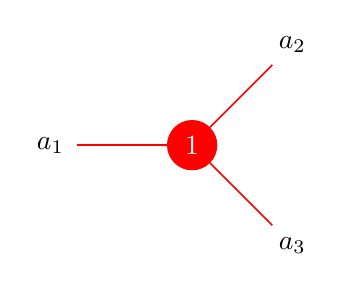
\begin{tikzpicture}[>=stealth',shorten >=1pt,auto,node distance=1.8cm,
                    semithick]
  \tikzstyle{every state}=[fill=red,draw=red,text=white,minimum size=5mm]

  \node[state] (1)                   {$1$};
  \node(a1)    [left of=1]           {$a_1$};
  \node(a2)    [above right of=1]    {$a_2$};
  \node(a3)    [below right of=1]    {$a_3$};
  \draw[red] 
        (1) edge              node {} (a1)
            edge              node {} (a2)
            edge              node {} (a3);
\end{tikzpicture}
\end{center}
the identity $f^{a_1 a_2 a_3} f^{a_1a_2a_4} = C_A \delta^{a_3a_4}$ corresponds to:
\begin{center}
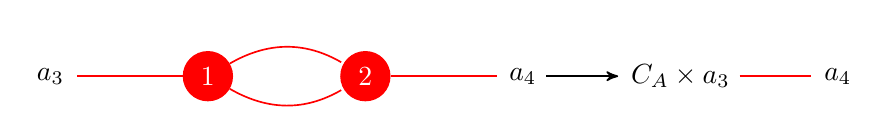
\begin{tikzpicture}[>=stealth',shorten >=1pt,auto,node distance=2cm,
                    semithick]
  \tikzstyle{every state}=[fill=red,draw=red,text=white,minimum size=5mm]

  \node[state] (1)                   {$1$};
  \node(a1)    [left of=1]           {$a_3$};
  \node[state] (2) [right of=1]      {$2$};
  \node(a2)    [right of=2]           {$a_4$};
  \draw[red] 
        (1) edge   [bend right]         node {} (2)
        (1) edge   [bend left]          node {} (2)
        (1) edge node {} (a1)
        (2) edge node {} (a2);
  \node (a3) [right of=a2] {$C_A\times a_3$};
  \node (a4) [right of=a3] {$a_4$};
  \draw[black,->] 
  (a2) edge node{} (a3);
  \draw[red]
  (a3) edge node{} (a4);
\end{tikzpicture}
\end{center}

The \texttt{FFLinks} correspond to the edges of the graphs, in terms of graphs the equivalence becomes, that two expressions are equivalent if they have the same graph. Our example has the corresponding graph:

\begin{center}
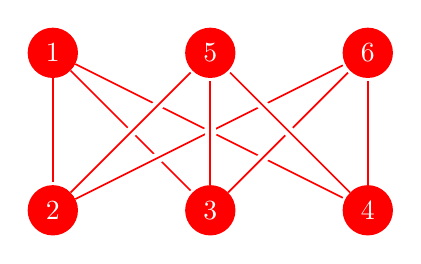
\begin{tikzpicture}[>=stealth',shorten >=1pt,auto,node distance=2cm,
                    semithick]
  \tikzstyle{every state}=[fill=red,draw=red,text=white,minimum size=5mm]

  \node[state] (1)                   {$1$};
  \node[state] (2) [below of=1]      {$2$};
  \node[state] (3) [right of=2]      {$3$};
  \node[state] (4) [right of=3]      {$4$};
  \node[state] (5) [right of=1]      {$5$};
  \node[state] (6) [right of=5]      {$6$};
  
  \draw[red] 
        (1) edge   [draw=white,double=red,double distance = \pgflinewidth,ultra thick]    node {} (2)
        (1) edge   [draw=white,double=red,double distance = \pgflinewidth,ultra thick]    node {} (3)
        (1) edge   [draw=white,double=red,double distance = \pgflinewidth,ultra thick]    node {} (4)
        (2) edge   [draw=white,double=red,double distance = \pgflinewidth,ultra thick]    node {} (5)
        (2) edge   [draw=white,double=red,double distance = \pgflinewidth,ultra thick]    node {} (6)
        (3) edge   [draw=white,double=red,double distance = \pgflinewidth,ultra thick]    node {} (5)
        (3) edge   [draw=white,double=red,double distance = \pgflinewidth,ultra thick]    node {} (6)
        (4) edge   [draw=white,double=red,double distance = \pgflinewidth,ultra thick]    node {} (5)
        (4) edge   [draw=white,double=red,double distance = \pgflinewidth,ultra thick]    node {} (6);
\end{tikzpicture}
\end{center}

this is the well-known bipartite graph $K_{3,3}$, the actual value of this graph is $0$. From now on we shall drop 
the labeling over the \FNodes, since the value of the grapsh is independent on this labeling. The relative spatial
possition of the nodes is also irrelevant for the value of the graph, for example the two graphs:

\begin{center}
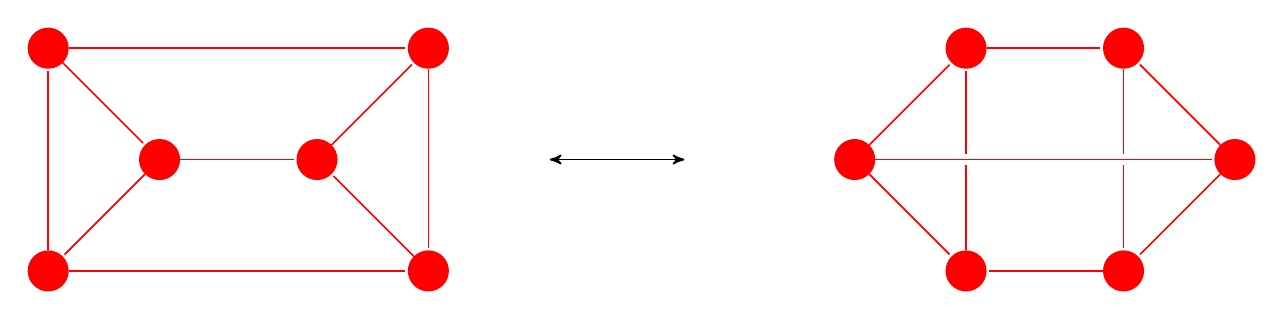
\begin{tikzpicture}[>=stealth',shorten >=1pt,auto,node distance=2cm,
                    semithick]
  \tikzstyle{every state}=[fill=red,draw=red,minimum size=5mm]

  \node[state] (1)                   {};
  \node[state] (2) [below left of=1]      {};
  \node[state] (3) [above left of=1]      {};
  \node[state] (4) [right of=1]      {};
  \node[state] (5) [above right of=4]      {};
  \node[state] (6) [below right of=4]      {};
  \node[] (G1) [below right of=5] {};
  
  \draw[red] 
        (1) edge   []         node {} (2)
        (2) edge   []         node {} (3)
        (3) edge   []         node {} (1)
        (1) edge   []         node {} (4)
        (2) edge   []         node {} (6)
        (3) edge   []         node {} (5)
        (4) edge   []         node {} (5)
        (5) edge   []         node {} (6)
        (6) edge   []         node {} (4);
  \node[] (G2) [right of=G1]{}; 
  \node[state] (7) [right of=G2]                {};
  \node[state] (8) [above right of=7]      {};
  \node[state] (9) [below right of=7]      {};
  \node[state] (10) [right of=8]      {};
  \node[state] (11) [right of=9]      {};
  \node[state] (12) [below right of=10]      {};
%   \node[state] (aux) [below right of=9]{};
  
  \draw[red] 
        (8) edge   []         node {} (10)
        (10) edge   []         node {} (11)
        (11) edge   []         node {} (9)
        (9) edge   []         node {} (8)
        (7) edge   []         node {} (8)
        (7) edge   []         node {} (9)
        (12) edge   []         node {} (10)
        (12) edge   []         node {} (11)
        (7) edge   [draw=white,double=red,double distance = \pgflinewidth,ultra thick] node {} (12);
  
  \draw[black,<->]
        (G1) edge node{}(G2);
\end{tikzpicture}
\end{center}

have the same value.

\subsection{Expression Classification using Graphs}
We now proceed to describe the classification procedure and how it is currently implemented in \texttt{NLOX}.
Graphs with only two nodes are evaluated down to a number trivially by the rules given in \eqref{}, so to start
we consider expressions with $4$ $f$ tensors, as we described before there is only one such strcture upon cannonical ordering, which is the tetrahedral graph:


\begin{center}
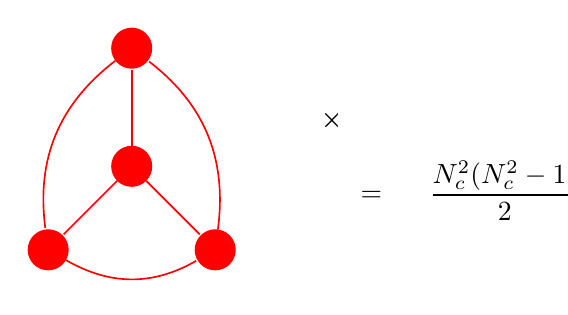
\begin{tikzpicture}[>=stealth',shorten >=0.5pt,auto,node distance=1.5cm,
                    semithick]
  \tikzstyle{every state}=[fill=red,draw=red,minimum size=5mm]
  \tikzstyle{equation} = [
    rectangle, rounded corners, inner sep=10pt, inner ysep=20pt]
  \node[state] (1)                   {};
  \node[state] (2) [above of=1]      {};
  \node[state] (3) [below left  of=1]      {};
  \node[state] (4) [below right of=1]      {};
  \node[] (Separator) [above right of=4]      {};
  \node[equation] (Value) [right of=Separator] {\begin{minipage}[ht!]{0.2\textwidth}
                                               ×\begin{equation*}
                                                   \hskip0.5cm =\hskip0.5cm  \frac{N_c^2(N_c^2-1)}{2}
                                                \end{equation*}
                                              \end{minipage}};
  \draw[red]
  (1) edge node{} (2)
  (1) edge node{} (3)
  (1) edge node{} (4)
  (2) edge [bend right]node{} (3)
  (3) edge [bend right]node{} (4)
  (4) edge [bend right]node{} (2);
  \end{tikzpicture}
\end{center}

for exprssions with $6$ \FNodes there are only $2$ possible graphs that are not trivially reduced to the tetrahedral graph, $K_{3,3}$ and the triangular prism graph shown above:

\begin{center}
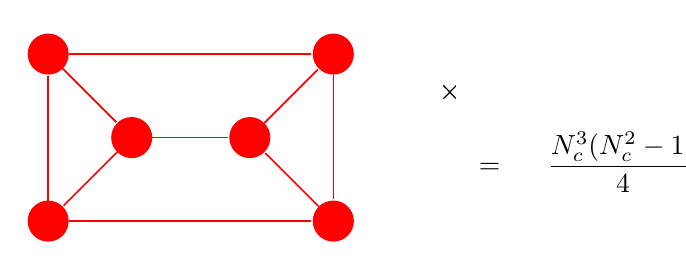
\begin{tikzpicture}[>=stealth',shorten >=0.5pt,auto,node distance=1.5cm,
                    semithick]
  \tikzstyle{every state}=[fill=red,draw=red,minimum size=5mm]
  \tikzstyle{equation} = [
    rectangle, rounded corners, inner sep=10pt, inner ysep=20pt]
  

  \node[state] (1)                   {};
  \node[state] (2) [below left of=1]      {};
  \node[state] (3) [above left of=1]      {};
  \node[state] (4) [right of=1]      {};
  \node[state] (5) [above right of=4]      {};
  \node[state] (6) [below right of=4]      {};
  \draw[red] 
        (1) edge   []         node {} (2)
        (2) edge   []         node {} (3)
        (3) edge   []         node {} (1)
        (1) edge   []         node {} (4)
        (2) edge   []         node {} (6)
        (3) edge   []         node {} (5)
        (4) edge   []         node {} (5)
        (5) edge   []         node {} (6)
        (6) edge   []         node {} (4);

  \node[] (Separator) [above right of=6]      {};
  \node[equation] (Value) [right of=Separator] {\begin{minipage}{0.2\textwidth}
                                               ×\begin{equation*}
                                                   \hskip0.5cm =\hskip0.5cm \frac{N_c^3(N_c^2-1)}{4}
                                                \end{equation*}
                                              \end{minipage}};
\end{tikzpicture}  
\end{center}

\begin{center}
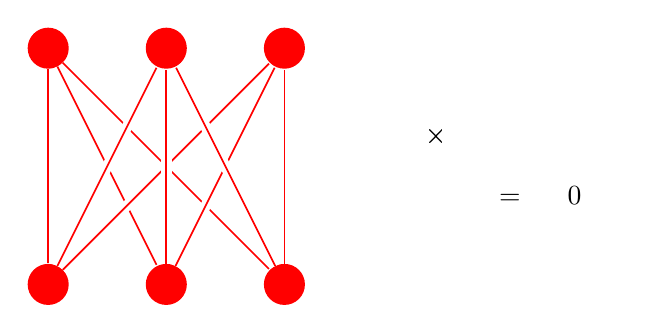
\begin{tikzpicture}[>=stealth',shorten >=0.5pt,auto,node distance=1.5cm,
                    semithick]
  \tikzstyle{every state}=[fill=red,draw=red,minimum size=5mm]
  \tikzstyle{equation} = [
    rectangle, rounded corners, inner sep=10pt, inner ysep=20pt]
  

  \node[state] (1){};
  
  \node[] (2B) [below of=1]      {};
  \node[state] (2) [below of=2B]      {};
  
  \node[state] (3) [right of=2]      {};
  \node[] (3B) [above of=3]      {};
  
  \node[state] (4) [right of=3]      {};
  \node[] (4B) [above of=4]      {};
  
  \node[state] (5) [right of=1]      {};
  \node[state] (6) [right of=5]      {};
  
  \draw[red] 
        (1) edge   [draw=white,double=red,double distance = \pgflinewidth,ultra thick]   node {} (2)
        (1) edge   [draw=white,double=red,double distance = \pgflinewidth,ultra thick]   node {} (3)
        (1) edge   [draw=white,double=red,double distance = \pgflinewidth,ultra thick]   node {} (4)
        (2) edge   [draw=white,double=red,double distance = \pgflinewidth,ultra thick]   node {} (5)
        (2) edge   [draw=white,double=red,double distance = \pgflinewidth,ultra thick]   node {} (6)
        (3) edge   [draw=white,double=red,double distance = \pgflinewidth,ultra thick]   node {} (5)
        (3) edge   [draw=white,double=red,double distance = \pgflinewidth,ultra thick]   node {} (6)
        (4) edge   [draw=white,double=red,double distance = \pgflinewidth,ultra thick]   node {} (5)
        (4) edge   [draw=white,double=red,double distance = \pgflinewidth,ultra thick]   node {} (6);
  \node[] (Separator) [right of=4B]      {};
  \node[equation] (Value) [right of=Separator] {\begin{minipage}{0.2\textwidth}
                                               ×\begin{equation*}
                                                   \hskip0.5cm =\hskip0.5cm 0
                                                \end{equation*}
                                              \end{minipage}};
\end{tikzpicture}  
\end{center}

while for $8$ \FNodes we 3 planar structures:
\begin{center}
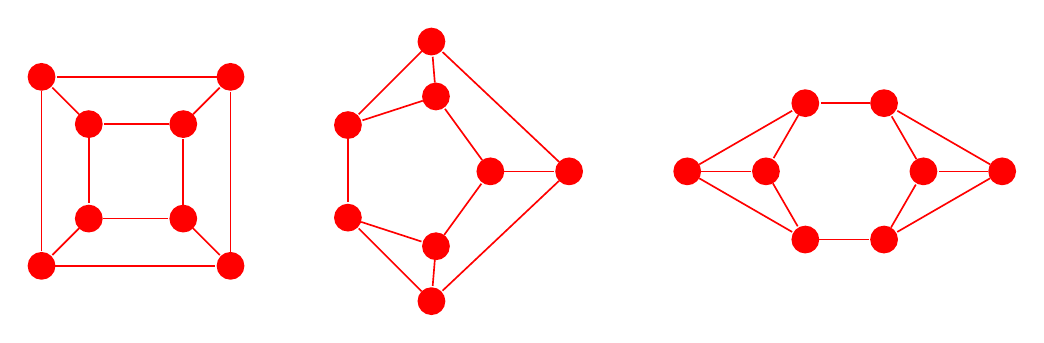
\begin{tikzpicture}[>=stealth',shorten >=0.5pt,auto,node distance=1.5cm,
                    semithick]
  \tikzstyle{every state}=[fill=red,draw=red,minimum size=3mm]
  \tikzstyle{equation} = [
    rectangle, rounded corners, inner sep=10pt, inner ysep=20pt]
  
  \node[]      (20) at (0,0) [] {};
  \node[state] (21) at ( 0.6, 0.6) [] {};
  \node[state] (22) at (-0.6, 0.6) [] {};
  \node[state] (23) at (-0.6,-0.6) [] {};
  \node[state] (24) at ( 0.6,-0.6) [] {};
  \node[state] (25) at ( 1.2, 1.2) [] {};
  \node[state] (26) at (-1.2, 1.2) [] {}; 
  \node[state] (27) at (-1.2,-1.2) [] {};
  \node[state] (28) at ( 1.2,-1.2) [] {};
  
  \draw[red] 
        (21) edge  node {} (22)
        (22) edge  node {} (23)
        (23) edge  node {} (24)
        (24) edge  node {} (21)
        (25) edge  node {} (26)
        (26) edge  node {} (27)
        (27) edge  node {} (28)
        (28) edge  node {} (25)
        (21) edge  node {} (25)
        (22) edge  node {} (26)
        (23) edge  node {} (27)
        (24) edge  node {} (28);
  
  \tikzset{shift={(3.5,0)}}
  
  \node[] at (0,0) [] {};
  \node[state] (1) at (1,0) [] {};
  \node[state] (2) at (0.3090,0.9510) [] {};
  \node[state] (3) at (-0.809017, 0.587785) [] {};
  \node[state] (4) at (-0.809017, -0.587785) [] {};
  \node[state] (5) at (0.3090,-0.9510) [] {};
  \node[state] (6) at (2,0) {};
  \node[state] (7) [above right of=3] {};
  \node[state] (8) [below right of=4] {};
  
  \draw[red] 
        (1) edge  node {} (2)
        (2) edge  node {} (3)
        (3) edge  node {} (4)
        (4) edge  node {} (5)
        (5) edge  node {} (1)
        (1) edge  node {} (6)
        (2) edge  node {} (7)
        (5) edge  node {} (8)
        (6) edge  node {} (7)
        (6) edge  node {} (8)
        (7) edge  node {} (3)
        (8) edge  node {} (4);
  
  
  \tikzset{shift={(5.5,0)}}
  \node[]      (10) at (0,0) [] {};
  \node[state] (11) at (1,0) [] {};
  \node[state] (12) at (0.5,0.866025) [] {};
  \node[state] (13) at (-0.5,0.866025) [] {};
  \node[state] (14) at (-1,0) [] {};
  \node[state] (15) at (-0.5,-0.866025)  [] {};
  \node[state] (16) at (0.5,-0.866025) [] {};
  \node[state] (17) at (2,0) {};
  \node[state] (18) at (-2,0) {};
  
  \draw[red] 
        (11) edge  node {} (12)
        (12) edge  node {} (13)
        (13) edge  node {} (14)
        (14) edge  node {} (15)
        (15) edge  node {} (16)
        (16) edge  node {} (11)
        (17) edge  node {} (11)
        (17) edge  node {} (16)
        (17) edge  node {} (12)
        (18) edge  node {} (14)
        (18) edge  node {} (15)
        (18) edge  node {} (13);
  
  
  \end{tikzpicture}  
\end{center}

\newpage
\section{Color Correlations}
Color correlated matrix elements are available in \NLOX as of ver \Placeholder.
The generation of color-correlated matrix elements is \texttt{off} per default, 
it can be activated via the input file by setting:\\

  \texttt{generateColorCorrelations = true}\\

For evaluation, there exists a One-Loop-Provider level function thal calls for their evaluation:\\

  \texttt{NLOX\_OLP\_EvalSubProcess\_CC(isub,type,cp,pp,next,mu,borncc,acc)}\\
  
  
\noindent which can only be called for Born matrix elements. 
The return pointer \texttt{borncc} must have a length of $1+\frac{n(n-1)}{2}$ where \texttt{NLOX} will store 
the uncorrelated born as well as all the pairwise color-correlated matrix elements in lexicographical order on the labels of the external particles, the first entry is reserved for the uncorrelated Born.\\

The implementation on the \texttt{FORM} code is done in \texttt{redefineFields.prc}, at this stage 
we replace the usual color contraction tensor that communicates the tree with the tree*, if no 
color-correlations are computed the tensor would be:

\begin{equation}
 (\mathcal{M}_0)^*(\tilde{\mathcal{M}_0}) = 
 \mathcal{M}_0^{c_1,...,c_n}\delta_{c_1d_1}\dots\delta_{d_1d_n}\tilde{\mathcal{M}}_0^{*d_1,...,d_n} 
 = \Big<\mathcal{M}_0\Big|\left|\mathcal{\tilde M}_0\right>
\end{equation}
where the $c$'s and $d$'s denote either fundamental or adjoint indices depending on the nature 
of the particle. We replace every intermediate tensor by:

\begin{equation}
 \delta_{c_id_i}\rightarrow \left(\text{ccL}_0\delta_{c_id_i}+ \text{ccLP }\text{ccL}_i (\textbf{T}^a)_{c_id_i}\right),
\end{equation}
the generator $\textbf{T}^a$ has different values depending on the nature of the particle:

  \[ 
  (\textbf{T}^a)_{c_id_i} =
  \begin{cases} 
      -(T^a)_{c_id_i} & \text{for initial quarks and final anti-quarks} \\
      (T^a)_{d_ic_i} & \text{for initial anti-quarks and final quarks} \\
      if^{c_id_ia} & \text{for gluons} 
   \end{cases}
  \]
To produce just the required correlations we throw away any term that does not have $0$ or
$2$ powers of ccLP, we also identify $\text{ccL}_0^2\rightarrow \text{ccL}_0$, $\text{ccLP}\rightarrow 1$ and 
$\text{ccL}_0\text{ ccL}_i\rightarrow \text{ccL}_i$, the final result for the color-correlated amplitude inside \NLOX is:

\begin{equation}
  \Big<\mathcal{M}_0\Big|\left|\mathcal{\tilde M}_0\right>_{CC} = 
 \text{ccL}_0 \Big<\mathcal{M}_0\Big|\left|\mathcal{\tilde M}_0\right> +  
 \sum_{i \neq j} \text{ccL}_i\text{ ccL}_j 
 \Big<\mathcal{M}_0\Big|\textbf{T}_i\textbf{T}_j\left|\mathcal{\tilde M}_0\right>.
\end{equation}

\newpage
\section{QCD and EW Real IR Poles}
\subsection{Implementation @NLOX}

Real IR-Pole routines are implemented within \NLOX, they are used 
for comparing them with the IR behaviour of the generated virtual 
amplitude and provide a stability check of the tensor reduction algorithm. 
The routines that use this IR pole stability checks are available at the 
One-Loop-Provider level via the function:\\

\texttt{NLOX\_OLP\_EvalSubProcess\_Alpha(isub,i,type,cp,pp,next,mu,rval2,acc)}\\

This function takes the same arguments as its non-Alpha counterpart except for the coupling-power
combination specification \texttt{cp} which is now expected to be in the format \texttt{cp = asXaeY},
where $X$ is the desired combined power of $\alpha_s$ and $Y$ is the desired combined power of $\alpha_e$.\\

The result of the Real-IR pole is computed alongside the Virtual-IR pole coming from the tensor reduction
procedure, as the LN Theorem states these two must cancel against each other to provide a finite 
final result. This fact can be used to provide a check on the stability of the tensor reduction 
algorithm since large differences point to numerical instabilities of the tensor reduction 
procedure. There is a user-accesible parameter \texttt{IR\_THRESHOLD} that sets the level 
of agreement required between the two IR-Poles for the phase-space-point to be considered safe,
the dafault behaviour is that \NLOX deems a phase-space-point unstable if less than \texttt{IR\_THRESHOLD} significant digits agree between the two IR-Poles. \\

\subsection{Master Formula}
To calculate the Real-IR Pole \NLOX uses a dipole subtraction inspired formula, essentially we 
compute the endpoint contribution of both the QCD and EW Dipoles applied to a particular LO 
interference, in what follows we will only consider processes that are not loop induced meaning 
that the leading order matrix elements are just a sum of tree level amplitudes:

\begin{equation}
 \left|\mathcal{M}_{0}\right> = \sum_{i,j}e^i g^j \left|\hat{\mathcal{M}}^{i,j}_{0}\right>
\end{equation}
and the differential cross section is a coupling-power convolution of tree matrix elements:

\begin{equation}
 \int d\sigma_{LO} = \int d\Phi_{n}
 \sum_{a,b} g^{a} e^{b}\sum_{i,j}
 \left<{\hat{\mathcal{M}}}^{i,j}_{0}\right|
 \left|{\hat{\mathcal{M}}}^{a-i,b-j}_{0}\right>
\end{equation}
where as to go higher one power in both $\alpha_s$ and $\alpha_e$ we must consider the 1-loop
matrix elements as well as trees with one extra external particle:

\begin{equation}
 \int d\sigma^V_{NLO} = 
 \int d\Phi_{n}\sum_{a,b}
 g^a e^b 
 \sum_{i,j}
 2\text{Re}\left[
 \MBra{0}{i}{j}
 \left(
  g^2\MKet{1}{a+2-i}{b-j}
 +
 e^2\MKet{1}{a-i}{b+2-j}
 \right)
 \right]
\end{equation}
the IR divergent part of the Real emission matrix element can be extracted analitycally in 
dimensional regularization using a dipole subtraction scheme, in it the poles are contained 
in the endpoint contributions of the QCD and EW dipoles:

\begin{equation}
 \int d\sigma^E_{NLO} = \int d\Phi_{n}
 \sum_{a,b} g^{a} e^{b} 
 \sum_{i,j}
 \MBra{0}{i}{j}
 \left(
 g^2\textbf{G}_{QCD}
 +
 e^2\textbf{G}_{EWK}
 \right)
 \MKet{0}{a-i}{b-j}
\end{equation}
we use bold names to indicate that the endpoint contributions are operators in color and spin space. 
These endpoint contributions contain both the real emission poles as well as the PDF counterterterm poles.
The two differential cross sections are compared order by order in perturbation theory and since:

\begin{equation}
 \int d\Phi_n \left(d\sigma_{NLO}^V + d\sigma_{NLO}^E\right) \sim \mathcal{O}(\epsilon^0),
 \label{cancellation}
\end{equation}
we expect the poles to be opposite in sign and cancel. As an example we show in tables~\ref{virt_uubar} and  \ref{real_uubar} the computed poles using both \TRed and the built-in endpoint contributions. 


\newgeometry{left=0.35in,right=1in}
\begin{table}[]
 \begin{tabular}{|c|c|c|c|c|c|c}\hline
 Order& Interference Type
 & \multicolumn{2}{c}{$1/\epsilon^{2}$} 
 & \multicolumn{2}{|c|}{$1/\epsilon$}\\\hline
 $\alpha_s^3$                           
 & 2Re$\left(\MBra{1}{4}{0}\MKet{0}{2}{0}\right)$
 & \multicolumn{2}{c|}{-18.2085841576369} 
 & \multicolumn{2}{c|}{-21.1265702280015} \\\hline
 \multirow{2}{*}{$\alpha_s^2\alpha_e$}                                                        
 & 2Re$\left(\MBra{1}{4}{0}\MKet{0}{0}{2}\right)$
 & 1.5055728821233 & \multirow{2}{*}{-3.0583822882991} 
 & 4.2169093557827 & \multirow{2}{*}{-17.7740636794077} \\
 & 2Re$\left(\MBra{1}{2}{2}\MKet{0}{2}{0}\right)$
 & -4.5639551704224 && -21.9909730351904 &\\\hline
 \multirow{2}{*}{$\alpha_s\alpha_e^2$}                                                  
 & 2Re$\left(\MBra{1}{2}{2}\MKet{0}{0}{2}\right)$
 & -21.6853196393154 & \multirow{2}{*}{-21.1834620119410} 
 & -94.6803519429044 & \multirow{2}{*}{-92.5133587992241} \\
 & 2Re$\left(\MBra{1}{0}{4}\MKet{0}{2}{0}\right)$
 & 0.5018576273744 && 2.1669931436803 &\\\hline
 $\alpha_e^3$                                                                             
 & 2Re$\left(\MBra{1}{0}{4}\MKet{0}{0}{2}\right)$
 & \multicolumn{2}{c|}{-7.3957257555633} 
 & \multicolumn{2}{c|}{-31.9343298391047} \\\hline
   \multicolumn{2}{|c|}{\textbf{Total}}     
 & \multicolumn{2}{c|}{\textbf{-49.8461542134402}} 
 & \multicolumn{2}{c|}{\textbf{-163.3483225457380}}\\\hline
 \end{tabular}
 \caption{Virtual IR Poles for $u\bar u\longrightarrow u\bar u$ using \TRed}
 \label{virt_uubar}
 
 
\vskip 0.75cm

 \begin{tabular}{|c|c|c|c|c|c|c|}\hline
 Order& Interference Type
 & \multicolumn{2}{c}{$1/\epsilon^{2}$} 
 & \multicolumn{2}{|c|}{$1/\epsilon$}\\\hline
 $\alpha_s^3$                           
 & $\MBra{0}{2}{0}\textbf{G}_{QCD}\MKet{0}{2}{0}$
 & \multicolumn{2}{|c|}{18.2085841576370} 
 & \multicolumn{2}{|c|}{21.1265702280016} \\\hline
 \multirow{2}{*}{$\alpha_s^2\alpha_e$}                                                        
 & 2Re$\left(\MBra{0}{2}{0}\textbf{G}_{QCD}\MKet{0}{0}{2}\right)$
 & -3.0111457642466 & \multirow{2}{*}{3.0583822882991} 
 & -8.4338187115655 & \multirow{2}{*}{-17.7740636794077} \\
 & $\MBra{0}{2}{0}\textbf{G}_{EWK}\MKet{0}{2}{0}$
 & 6.0695280525457 && 26.2078823909731 &\\\hline
 \multirow{2}{*}{$\alpha_s\alpha_e^2$}                                                  
 & $\MBra{0}{0}{2}\textbf{G}_{QCD}\MKet{0}{0}{2}$
 & 22.1871772666898 & \multirow{2}{*}{21.1834620119409} 
 & 96.8473450865848 & \multirow{2}{*}{92.5133587992241} \\
 & 2Re$\left(\MBra{0}{0}{2}\textbf{G}_{EWK}\MKet{0}{2}{0}\right)$ 
 & -1.0037152547489 && -4.3339862873607 &\\\hline
 $\alpha_e^3$                                                                             
 & $\MBra{0}{0}{2}\textbf{G}_{EWK}\MKet{0}{0}{2}$
 & \multicolumn{2}{|c|}{7.3957257555633} 
 & \multicolumn{2}{|c|}{31.9343298391050} \\\hline
   \multicolumn{2}{|c|}{\textbf{Total}}     
 & \multicolumn{2}{|c|}{\textbf{49.8461542134403}} 
 & \multicolumn{2}{|c|}{\textbf{163.3483225457380}}\\\hline
 \end{tabular}
 \caption{Real IR Poles for $u\bar u\longrightarrow u\bar u$ using the dipole subtraction formalism.}
 \label{real_uubar}

\footnotesize
\newgeometry{left=0.5in,right=0.5in}
\vskip0.75cm
\begin{tabular}{|c|c|c|c|c|c|c}\hline
 Order& Interference Type
 & \multicolumn{2}{c}{$1/\epsilon^{2}$} 
 & \multicolumn{2}{|c|}{$1/\epsilon$}\\\hline
 $\alpha_s^3$                           
 & 2Re$\left(\MBra{0}{2}{0}\frac{1}{2}\textbf{G}_{QCD}\MKet{0}{2}{0}\right)$
 & \multicolumn{2}{c|}{18.2085841576369} 
 & \multicolumn{2}{c|}{21.1265702280015} \\\hline
 \multirow{2}{*}{$\alpha_s^2\alpha_e$}                                                        
 & 2Re$\left(\MBra{0}{2}{0}\frac{1}{2}\textbf{G}_{QCD}\MKet{0}{0}{2}\right)$
 & -1.5055728821233 & \multirow{2}{*}{3.0583822882991} 
 & -4.2169093557827 & \multirow{2}{*}{17.7740636794077} \\
 & 2Re$
 \left(\left[
 \MBra{0}{0}{2}\frac{1}{2}\textbf{G}_{QCD}
 +
 \MBra{0}{2}{0}\frac{1}{2}\textbf{G}_{EWK}
 \right]
 \MKet{0}{2}{0}\right)$
 & 4.5639551704224 && 21.9909730351904 &\\\hline
 \multirow{2}{*}{$\alpha_s\alpha_e^2$}                                                  
 & 2Re$
 \left(\left[
 \MBra{0}{0}{2}\frac{1}{2}\textbf{G}_{QCD}
 +
 \MBra{0}{2}{0}\frac{1}{2}\textbf{G}_{EWK}
 \right]
 \MKet{0}{0}{2}\right)$
 & 21.6853196393154 & \multirow{2}{*}{21.1834620119409} 
 & 94.6803519429044 & \multirow{2}{*}{92.5133587992241} \\
 & 2Re$\left(\MBra{0}{0}{2}\frac{1}{2}\textbf{G}_{EWK}\MKet{0}{2}{0}\right)$
 & -0.5018576273744 && -2.1669931436803 &\\\hline
 $\alpha_e^3$                                                                             
 & 2Re$\left(\MBra{0}{0}{2}\frac{1}{2}\textbf{G}_{EWK}\MKet{0}{0}{2}\right)$
 & \multicolumn{2}{c|}{7.3957257555633} 
 & \multicolumn{2}{c|}{31.9343298391050} \\\hline
   \multicolumn{2}{|c|}{\textbf{Total}}     
 & \multicolumn{2}{c|}{\textbf{49.8461542134403}} 
 & \multicolumn{2}{c|}{\textbf{163.3483225457380}}\\\hline
 \end{tabular}
 \caption{Real IR Poles for $u\bar u\rightarrow u\bar u$, using dipole subtraction with 1-loop amplitudes
 disentangled.}
 \label{1loop_disentangled}
\end{table}
\restoregeometry

\subsection{1-loop Matrix element disentanglement}
The cancellation of the IR divergences must be fullfilled at fixed order on square amplitudes,
where the real and virtual matrix elemants can be combined, as shown on the rows of tasbles \ref{virt_uubar}
and \ref{real_uubar}. Alternatively one might attempt to check for the IR pole cancellation 
for a particular interference term on the virtual NLO cross section, this is also possible and 
we will discuss how we do it inside \NLOX. In general the IR behaviour of any given 1-loop amplitude 
is given by the sum of endpoint contributions:

\begin{equation}
 \MKet{1}{X}{Y} \rightarrow -\frac{1}{2}
 \left(
 \textbf{G}_{QCD}\MKet{0}{X-2}{Y} 
 + 
 \textbf{G}_{EWK}\MKet{0}{X}{Y-2}
 \right),
 \label{Theo}
\end{equation}
meaning that the squared amplitude built by using the sum on the RHS yields the opposite IR poles as the 
one built using the LHS as shown in tables \ref{virt_uubar} \ref{1loop_disentangled}. 
To prove that this holds true in general we have to evaluate \eqref{cancellation} order by order in 
perturbation theory, the result for the virtuals is:

\begin{equation}
 \int d\sigma^V_{NLO} = 
 \int d\Phi_{n}\sum_{a,b}
 g^a e^b 
 \sum_{i,j}
 2\text{Re}\left[
 \left(
  g^2\MBra{}{}{}
 +e^2\MBra{}{}{}
 \right)
 \left|{\hat{\mathcal{M}}}^{a-i,b-j}_{0}\right>
 \right]
\end{equation}



\begin{equation}
 \MKet{1}{X_0+2}{Y_0} \rightarrow -\frac{1}{2}
 \left(
 \textbf{G}_{QCD}\MKet{0}{X_0}{Y_0} 
 + 
 \textbf{G}_{EWK}\cancelto{0}{\MKet{0}{X_0+2}{Y_0-2}}
 \right),
 \label{boundary}
\end{equation}
since the second term vanishes, this statement is identical to \eqref{cancellation} when evaluated at the maximum power of $g$. Now we proceed to prove \eqref{Theo} by induction, we assume that for every $n<m-1$ the statement:
\begin{equation}
  \MKet{1}{X_0-2(n-1)}{Y_0+2n}\rightarrow -\frac{1}{2}
  \left(
  \textbf{G}_{QCD}\MKet{0}{X_0-2n}{Y_0+2n} 
 + 
 \textbf{G}_{EWK}\MKet{0}{X_0-2(n-1)}{Y_0+2(n-1)}
 \right)
\end{equation}
holds and use \eqref{cancellation} to prove that it must hold for $n=m$. Using \eqref{cancellation} at fixed 
order of $g^{2X_0+2(m-1)}e^{2Y_0+2m}$ we have:

\begin{equation}
 \Int{\Phi_n} \sum_{i,j}2\text{Re}\left[\right]\MKet{0}{2X_0-2(m-1)-i}{2Y_0+2m-j}
\end{equation}




\section{Spin-Correlated Amplitudes}
Spin correlated amplitudes are necessary for building the subtraction function they arise because 
we need to consider external off-shell photons and gluons in order to correctly capture the 
radiative matrix element's behaviour. The dipole functions are:

\begin{equation}
 P_{q\rightarrow gg} = 
\end{equation}




\end{document}
